% !TEX root = Projektdokumentation.tex
\section{Beispiel 2}
\label{sec:beispiel2}

\subsection{Ausgangssituation} 
\label{sec:ausgangssituation2}
Als Ausgangsmethode kann, wie in Beispiel 1 \ref{sec:ausgangssituation1}, wieder eine Wahl eines Kurssprechers angenommen werden. 

In dieser Wahl haben 21 Personen die Kandidaten $a$ bis $d$ in eine Reihenfolge sortiert.

\begin{description}
\centering
\item[8 mal] $a \succ_{v} c \succ_{v} d \succ_{v}b$
\item[2 mal] $b \succ_{v} a \succ_{v} d \succ_{v}c$
\item[4 mal] $c \succ_{v} d \succ_{v} b \succ_{v}a$
\item[4 mal] $d \succ_{v} b \succ_{v} a \succ_{v}c$
\item[3 mal] $d \succ_{v} c \succ_{v} b \succ_{v}a$
\end{description}



\subsection{Lösungsschritte} 
\label{sec:loesungen2}
Zuerst werden die Kandidaten wieder gegeneinander aufgestellt.

 \begin{description}
 \centering
 \item[$a$ vs. $b$] 8 Stimmen gegen 13 Stimmen, $b$ gewinnt
 \item[$a$ vs. $c$] 14 Stimmen gegen 7 Stimmen, $a$ gewinnt
 \item[$a$ vs. $d$] 10 Stimmen gegen 11 Stimmen, $d$ gewinnt
 \item[$b$ vs. $c$] 6 Stimmen gegen 15 Stimmen, $c$ gewinnt
 \item[$b$ vs. $d$] 2 Stimmen gegen 19 Stimmen, $d$ gewinnt
 \item[$c$ vs. $d$] 12 Stimmen gegen 9 Stimmen, $c$ gewinnt
 \end{description}
 
In diesem Fall sieht man, dass es keinen \condorcetSieger gibt, also keiner es geschafft hat alle Gegner im Zweikampf zu überholen, diese Situation ist das sogenannte \condorcetParadox. \citep{EnricoSchoebel2018}

Die \schulze kann diese Problem jedoch lösen indem, wie in Tabelle \ref{beispiel2_N} dargestellt, die Menge $N$ gebildet wird.

% !TEX root = Projektdokumentation.tex

\begin{longtable}[c]{|l|l|l|l|l|}
\hline
            & N{[}*,a{]} & N{[}*,b{]} & N{[}*,c{]} & N{[}*,d{]} \\ \hline
\endfirsthead
%
\endhead
%
N{[}a, *{]} & ---        & 8          & 14         & 10         \\ \hline
N{[}b, *{]} & 13         & ---        & 6          & 2          \\ \hline
N{[}c, *{]} & 7          & 15         & ---        & 12         \\ \hline
N{[}d, *{]} & 11         & 19         & 9          & ---        \\ \hline
\caption{Die Menge $N$ (Beispiel 2)}
\label{beispiel2N}\\
\end{longtable}

Aus der Menge $N$ wird der Graph \ref{fig:graph2} erstellt.

\begin{figure}[!h]
\centering
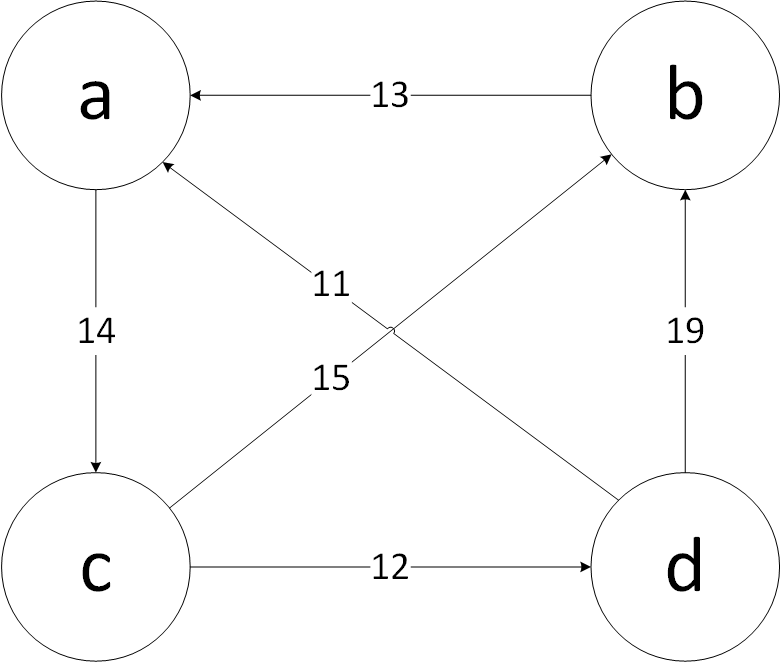
\includegraphics[scale=0.5]{Bilder/Beispiel2_Graph.png}
\caption{Graph über die Menge $N$}
\label{fig:graph2}
\end{figure}

Nun werden wieder die stärksten Pfade gesucht und in die Menge $P$ eingefügt, die in Tabelle \ref{beispiel2p} zu sehen ist.

% !TEX root = ../Projektdokumentation.tex

\begin{longtable}[c]{|l|l|l|l|l|}
\hline
             & P{[}*,a{]} & P{[}*,b{]} & P{[}*,c{]} & P{[}*,d{]} \\ \hline
\endfirsthead
%
\endhead
%
PN{[}a, *{]} & ---        & 14         & 14         & 12         \\ \hline
PN{[}b, *{]} & 13         & ---        & 13         & 12         \\ \hline
P{[}c, *{]}  & 13         & 15         & ---        & 12         \\ \hline
P{[}d, *{]}  & 13         & 19         & 13         & ---        \\ \hline
\caption{Die Menge $P$ in Beispiel 2}
\label{beispiel2p}\\
\end{longtable}

Anschließend wird mit den Werten der Menge $P$ die neu Zweikampfsituation erstellt und man erhält die Relation $\mathcal{O} = \{ ab,ac,cb,da,db,dc \}$


\subsection{Ergebnis} 
\label{sec:ergebnis2}
Analog zu Beispiel 1 (Abschnitt \ref{sec:beispiel1}) wird die Relation $\mathcal{O}$ untersucht um die Menge der Sieger zu finden. In diesem Fall ist $\mathcal{S}=\{d\}$  und der Sieger ist Kandidat d. Hier sieht man, dass die \schulze Probleme anderer Wahlverfahren lösen kann.

Eine Ausführliche Besprechung wie in Beispiel 1 kann in der orginal Ausarbeitung von Martin Schulze nachgelesen werden. \citep{Schulze2017}
